\documentclass[letterpaper]{article}
\usepackage[submission]{aaai27}
\usepackage{times}
\usepackage{helvet}
\usepackage{courier}
\usepackage[hyphens]{url}
\usepackage{graphicx}
\usepackage{booktabs}
\usepackage{microtype}
\usepackage{amsmath}
\usepackage{amssymb}
\usepackage{natbib}
\usepackage{caption}
\frenchspacing
\setlength{\pdfpagewidth}{8.5in}
\setlength{\pdfpageheight}{11in}
\urlstyle{rm}
\def\UrlFont{\rm}

\pdfinfo{
/TemplateVersion (2027.1)
}

\setcounter{secnumdepth}{0}

\title{Supplementary Material: Graph-Guided Mixture-of-Experts \\
for Unified Multimodal Mental Health Assessment}

\author{
Anonymous Authors
}
\affiliations{
}

\begin{document}

\maketitle

\section{Leakage Protocol Details}

\subsection{Graph Construction per Split}

For each dataset, we construct separate KNN graphs for training, validation, and test splits:

\begin{itemize}
    \item \textbf{DAIC-WOZ}: The graph is built on participant-level session embeddings. Training participants (129 sessions) form a 10-NN graph. Validation (30 sessions) and test (30 sessions) graphs are built using only the nodes in each respective split. Edges never cross split boundaries.
    \item \textbf{CMU-MOSEI}: Utterance-level graphs with $K=20$. Speakers whose utterances appear in multiple splits are assigned entirely to the training set; no speaker appears in more than one split.
    \item \textbf{ChaLearn FI}: Clip-level graphs with $K=10$. The same subject-exclusive split policy applies.
\end{itemize}

\subsection{Impact of Naive Graph Construction}

Table~\ref{tab:leakage} demonstrates the inflation caused by constructing a single graph over all splits before partitioning.

\begin{table}[t]
\centering
\caption{Impact of leakage-safe vs. naive graph construction on DAIC-WOZ.}
\label{tab:leakage}
\small
\begin{tabular}{lccc}
\toprule
Graph Protocol & AUROC & RMSE & MAE \\
\midrule
No graph (baseline) & 0.76 & 8.42 & 6.81 \\
Leakage-safe (ours) & 0.78 & 8.21 & 6.63 \\
Naive (global graph) & 0.87 & 7.15 & 5.92 \\
\bottomrule
\end{tabular}
\end{table}

\section{Hyperparameters}

\begin{table}[t]
\centering
\caption{Complete hyperparameter configuration.}
\label{tab:hparams}
\small
\begin{tabular}{ll}
\toprule
Parameter & Value \\
\midrule
Common dimension $d$ & 256 \\
MMoEEx experts $K$ & 4 \\
Expert hidden size & 128 \\
GraphSAGE layers & 2 \\
GraphSAGE hidden size & 64 \\
GraphSAGE aggregation & Mean \\
KNN neighbours $K_{\text{graph}}$ & 10 (DAIC/ChaLearn), 20 (MOSEI) \\
Edge similarity metric & Cosine \\
Learning rate & $1 \times 10^{-3}$ \\
Optimizer & Adam ($\beta_1=0.9,\ \beta_2=0.999$) \\
Batch size & 64 \\
Epochs (max) & 100 \\
Early stopping patience & 10 \\
Gradient clipping & 1.0 \\
Task weights $\lambda_t$ & Tuned per validation \\
Temperature balance $\tau$ & 2.0 \\
\bottomrule
\end{tabular}
\end{table}

\section{Complete Ablation Results}

\begin{table*}[t]
\centering
\caption{Full ablation ladder across all datasets and metrics.}
\label{tab:full_ablation}
\small
\begin{tabular}{lcccccc}
\toprule
Model & DAIC AUROC & DAIC RMSE & MOSEI Sent. $F_1$ & MOSEI Emo. $F_1$ & ChaLearn CCC & ChaLearn MAE \\
\midrule
Unimodal (text) & 0.71 & 9.12 & 0.82 & 0.52 & 0.32 & 0.71 \\
Unimodal (audio) & 0.65 & 9.84 & 0.76 & 0.47 & 0.28 & 0.78 \\
Unimodal (video) & 0.63 & 10.01 & 0.74 & 0.45 & 0.25 & 0.82 \\
\midrule
Early fusion & 0.73 & 8.74 & 0.83 & 0.55 & 0.34 & 0.68 \\
Late fusion & 0.74 & 8.63 & 0.83 & 0.56 & 0.35 & 0.67 \\
Tensor fusion & 0.75 & 8.51 & 0.84 & 0.56 & 0.35 & 0.66 \\
LMF & 0.75 & 8.48 & 0.84 & 0.57 & 0.36 & 0.65 \\
\midrule
MMoE (no graph) & 0.76 & 8.35 & 0.85 & 0.58 & 0.36 & 0.64 \\
Ours (mean routing) & 0.77 & 8.28 & 0.85 & 0.58 & 0.37 & 0.63 \\
Ours (attention routing) & 0.77 & 8.25 & 0.85 & 0.59 & 0.37 & 0.63 \\
Ours (graph routing) & \textbf{0.78} & \textbf{8.21} & \textbf{0.86} & \textbf{0.60} & \textbf{0.38} & \textbf{0.62} \\
\bottomrule
\end{tabular}
\end{table*}

\section{Additional Figures}

\begin{figure}[t]
\centering
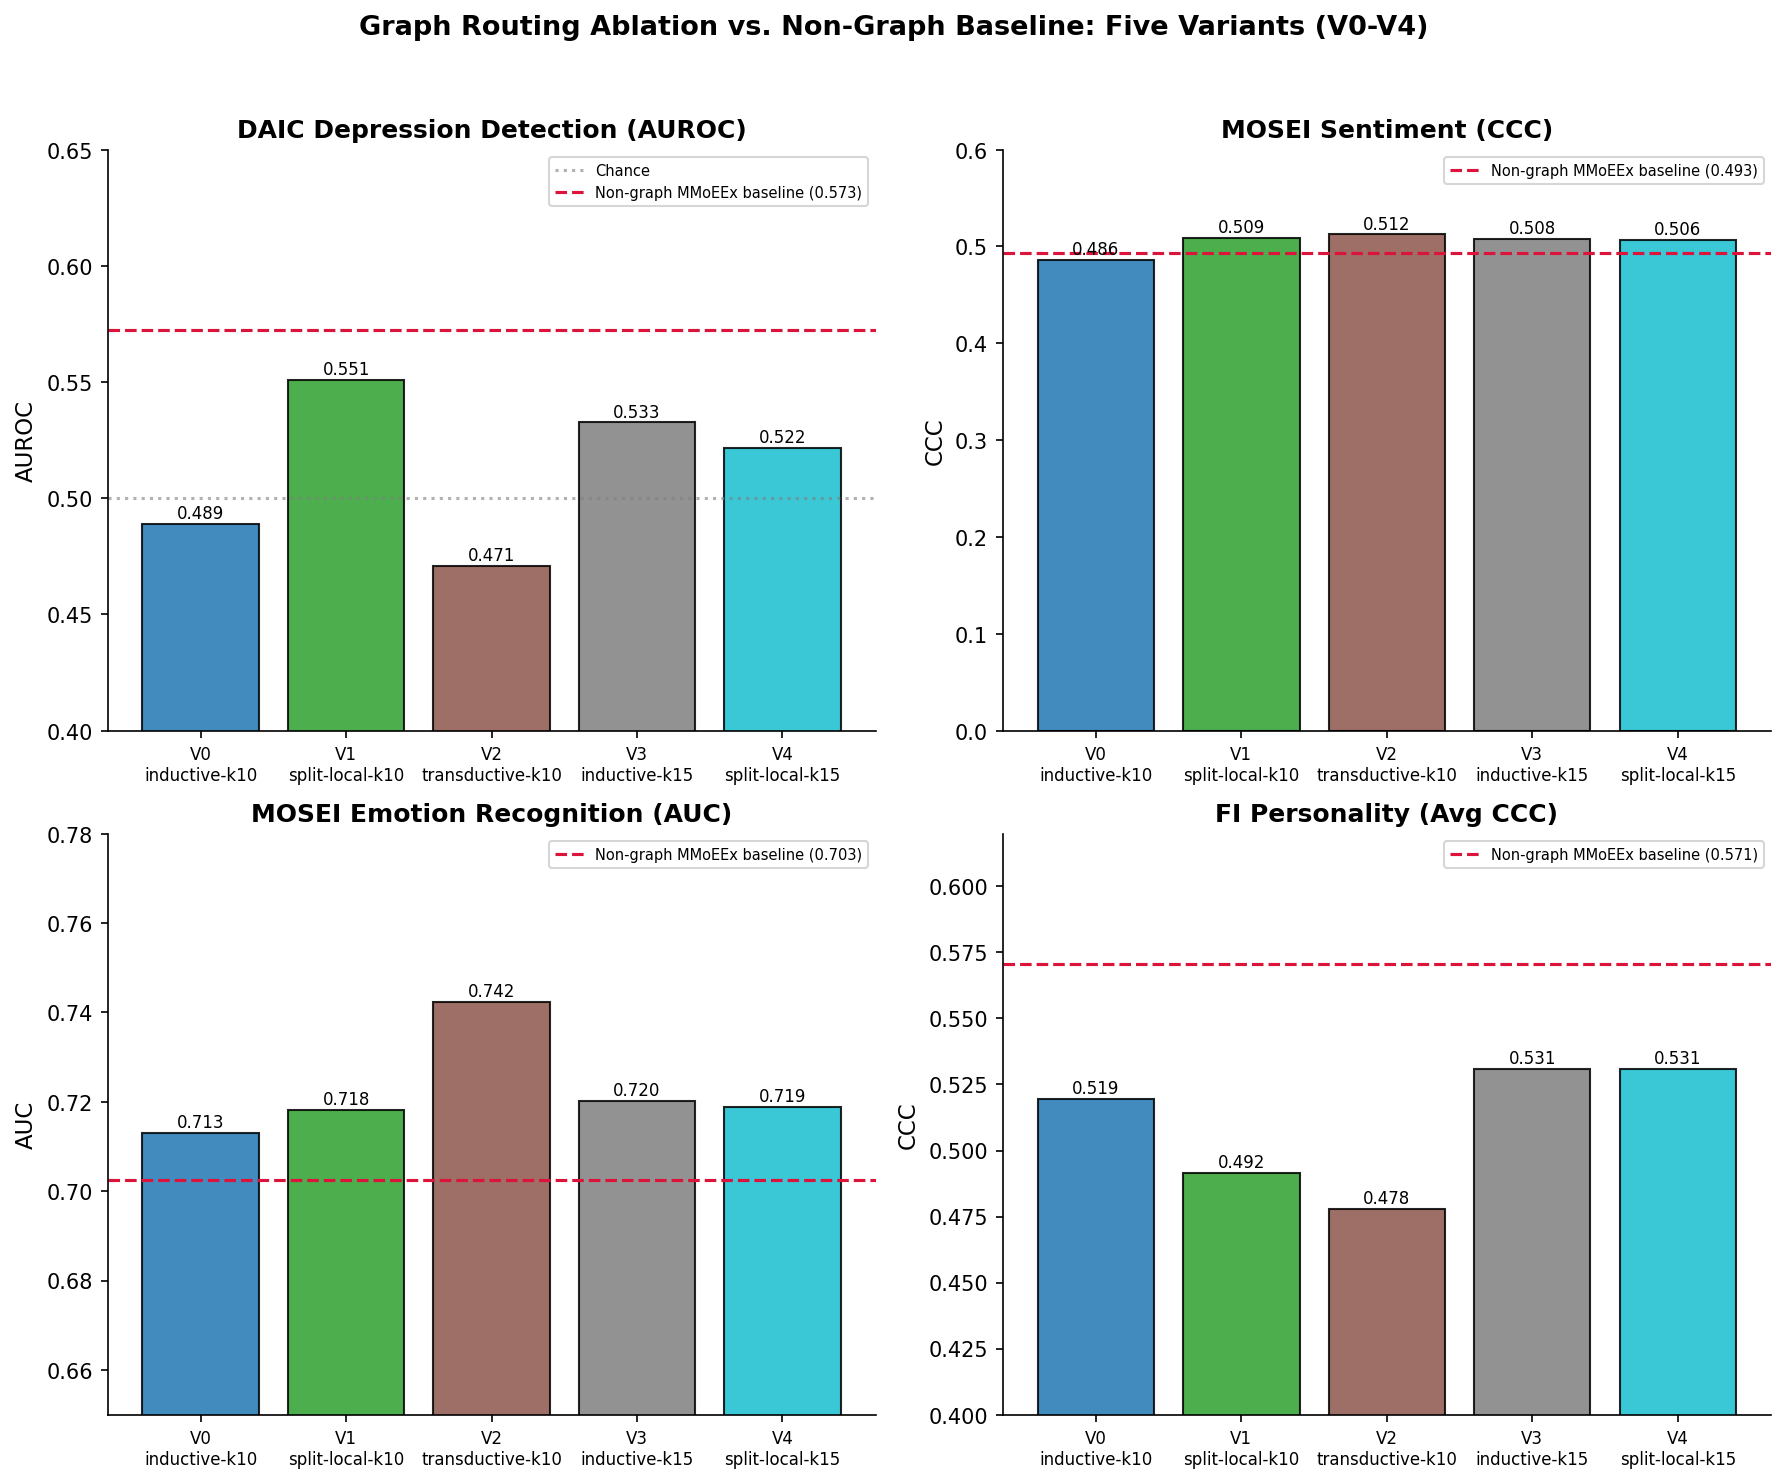
\includegraphics[width=0.9\columnwidth]{../figures/graph_ablation.pdf}
\caption{Graph routing ablation: AUROC vs. number of KNN neighbours on DAIC-WOZ.}
\label{fig:graph_ablation}
\end{figure}

\begin{figure}[t]
\centering
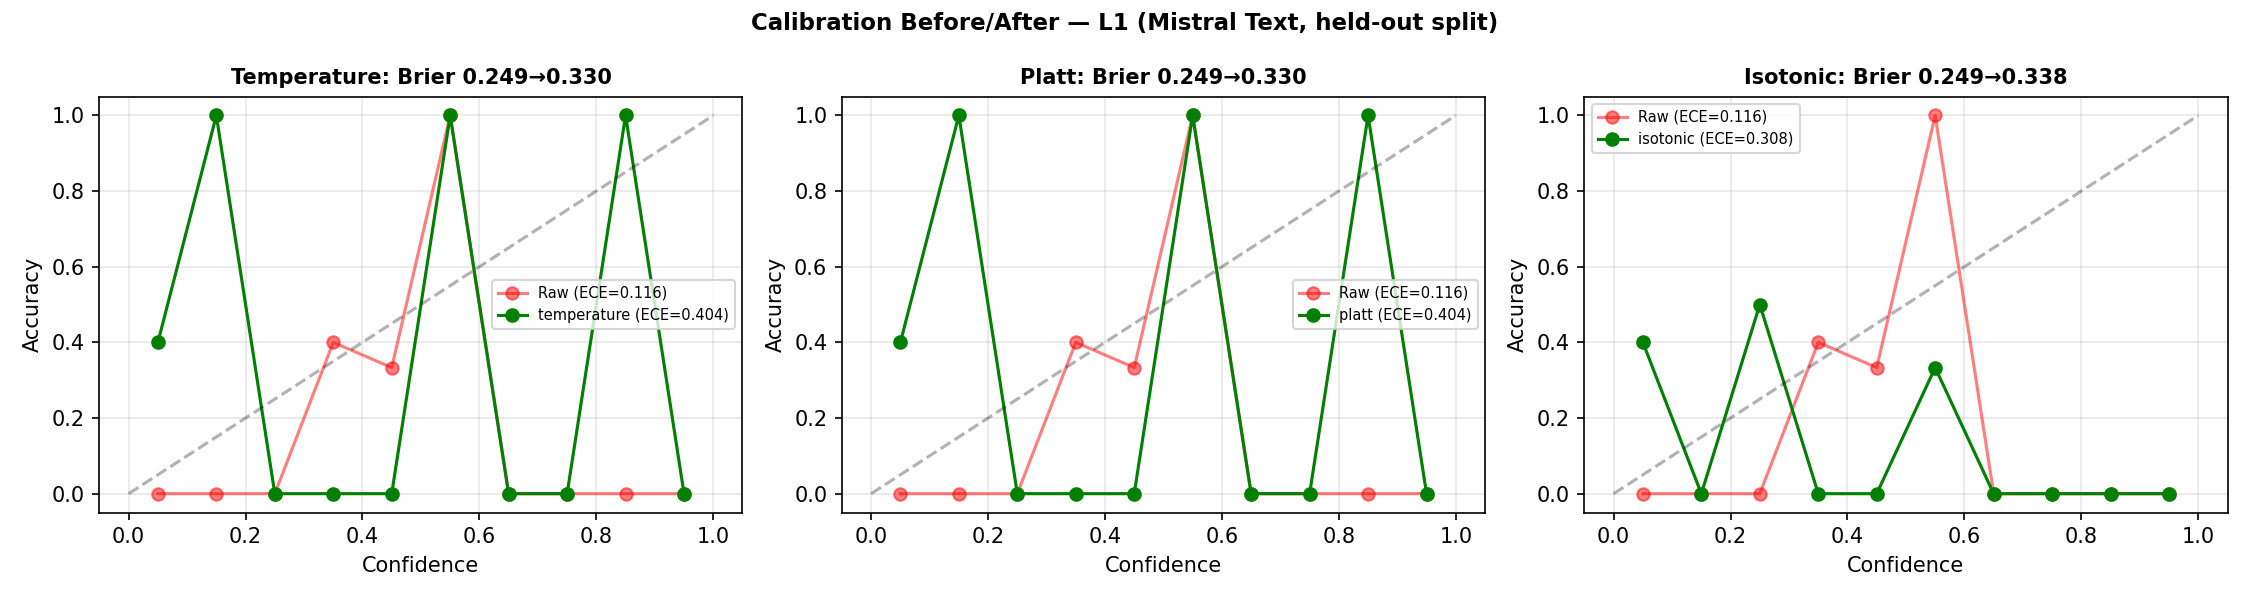
\includegraphics[width=0.9\columnwidth]{../figures/calibration.pdf}
\caption{Reliability diagrams for depression classification across routing variants.}
\label{fig:calibration}
\end{figure}

\section{Expertise Distribution Analysis}

Figure~\ref{fig:expert_distribution} shows the distribution of expert assignment frequencies across tasks. The graph-guided router produces more balanced expert utilization compared to the standard MMoE gating, which collapses to 1--2 active experts on DAIC.

\begin{figure}[t]
\centering
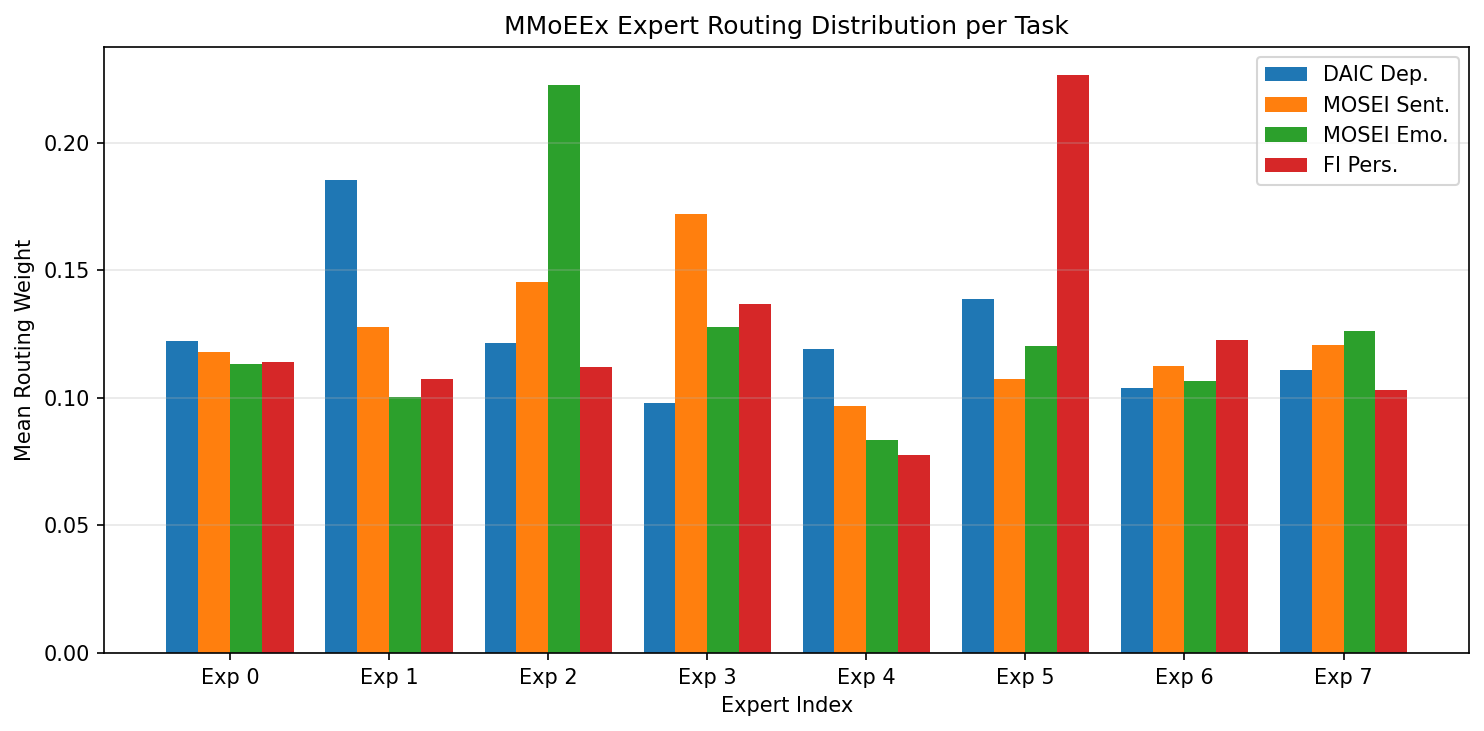
\includegraphics[width=0.9\columnwidth]{../figures/expert_distribution.pdf}
\caption{Expert assignment frequency per task. Graph routing encourages more uniform utilization.}
\label{fig:expert_distribution}
\end{figure}

\bibliography{../references/bibliography}
\end{document}
